\chapter{Event Reconstruction}\label{chap:reco}
	Before any physics analysis can be performed on the raw data from the \gls{ATLAS} detector or \gls{MC} simulations the raw datasets go through a reconstruction software suite called Athena \cite{athena}. Various algorithms are employed to identify energy deposits as particles based on shower shapes, tracker hits, calculated charge to mass ratios, etc. Figure \ref{fig:ATLAS-XSec} shows the signatures of various particles within the \gls{ATLAS} detector. 

	\begin{figure}[!ht]
	\centering
	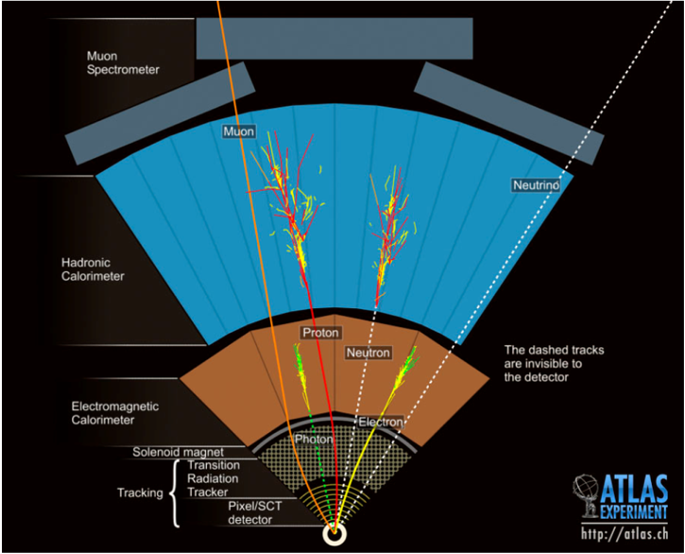
\includegraphics[width=.65\textwidth,keepaspectratio=true]{chapters/chapter3_experiment/images/ATLASCrossSectionDiagram.png}
	\caption{ Cross section view of the \gls{ATLAS} detector with subdetectors labeled. Various types of particles radial trajectories are shown \cite{atlas-experiment}.}
	\label{fig:ATLAS-XSec}
	\end{figure}

	The following sections detail the identification processes of muons, electrons, photons, jets, $\tau$ leptons, and a calculated quantity called missing transverse energy (\Etm). These reconstructed physics objects are the inputs to the majority of physics analyses.

	\section{Tracks}
		Tracks are fit-connected three-dimensional space-points in the \gls{ID}. These space-points are created from clusters of hits in the \gls{ID}. A set of three space-points are combined into one track seed, then fed into three methods in the \gls{ATLAS} detector: inside-out,  outside-in, and \gls{TRT}-standalone. The inside-out method creates tracks by starting with a seed hit in the pixel detector, then \gls{SCT} hits are added, finally the track is extrapolated out into the TRT. This method creates tracks of particles that are mostly produced in the hard \pp interaction and has a requirement of $\pt>400$ MeV. On the other-hand the outside-in method starts with track segments in the \gls{TRT} and extrapolates towards the beamline using silicon that were not used in the inside-out method. Outside-in tracking typically reconstructs secondary vertices from particles that have long enough lifetimes to decay while inside the \gls{ID}, including b quarks and $\tau$ leptons. Lastly, \gls{TRT}-standalone tracks are made only from seeds within the \gls{TRT} and are not extrapolated to the silicon subdetectors \cite{ATLAS-perf-run2}. The reconstructed tracks are used in the identification of various types of particles.

		% Reconstructed tracks are made at two working points (WPs) to give analyzers a variety of track fits to best fit the analysis' needs
		% \begin{multicols}{2}
		% \begin{itemize}
		% 	\item Loose
		% 	\begin{itemize}
		% 		\item $\pt > 400$ MeV
		% 		\item $|\eta|<2.5$
		% 		\item $\geq 7$ silicon hits
		% 		\item $\leq 1$ shared modules
		% 		\item $\leq 2$ silicon holes
		% 		\item $\leq 1$ pixel holes
		% 	\end{itemize}
		% 	\item Tight
		% 	\begin{itemize}
		% 		\item if $|\eta|<1.65$
		% 		\begin{itemize}
		% 			\item $\geq 9$ silicon hits
		% 		\end{itemize}
		% 		\item if $|\eta| > 1.65$
		% 		\begin{itemize}
		% 			\item $\geq 11$ silicon hits
		% 			\item 1 hit on 2 innermost pixel layers
		% 			\item 0 pixel holes
		% 		\end{itemize}
		% 	\end{itemize}
		% \end{itemize}	

		% \end{multicols}

	\section{Topological Clusters}
		A topocluster is defined as a cluster of topologically connected calorimeter cell signals. Topological clusters in the \gls{ATLAS} detector's calorimeters are vital to the identification of hadronic final states, meaning jets (Section \ref{sec:reco-jets}), isolated hadrons, and hadronically decaying $\tau$ leptons (Section \ref{ssec:reco-tau}). Topoclusters are also included in the calculation of missing transverse energy discussed in Section \ref{sec:reco-etmiss}, as they represent the direction and energy of softer particles in a collision event. 

		A topocluster is created via a growing volume algorithm that operates based on a set of three thresholds. These thresholds are defined using the calorimeter cell significance $\xi_{cell}$ \cite{topocluster-perf}:
		\begin{equation}
		\xi_{cell} = \frac{E_{cell}}{\sigma_{noise, cell}}
		\end{equation}
		where $E_{cell}$ is the energy in the calorimeter cell and $\sigma_{noise, cell}$ is the average expected noise of a given calorimeter cell. An in-depth review of how the $\sigma_{noise, cell}$ value is calculated for TileCal is given in Appendix \ref{app:Tile-DQ}. A topocluster starts with a seed cell that has a significance greater than the seed threshold S. From the seed cell, all three-dimensionally neighboring cells with a significance greater than the growth threshold N are added to the topocluster. This is done repeatedly until there are no more neighboring cells that pass the requirement $|\xi_{cell}|>N$. If a neighboring cell also passes the $|\xi_{cell}|>S$ threshold, then the topocluster corresponding to the neighbor cell is merged into the original topocluster. Finally, a last layer of the topocluster is added from all neighboring cells passing a threshold of $|\xi_{cell}|>P$. In the \gls{ATLAS} experiment, the threshold values are set at $(S,N,P) = (4,2,0)$.

		\section{Muon Identification}\label{sec:reco-muon}
		Muons are identified using a combination of information from the \gls{ID} and the \gls{MS}. Within the \gls{ID}, muons leave tracks identical to any other charged particle; however, in the \gls{MS} tracks are identified within the MDTs through a straight-line fit in a single layer and by doing a combinatorial search of CSC hits in the $\eta-\phi$ plane. \cite{muon-id} Muons are identified through five strategies, each using the information from the \gls{ID}, \gls{MS}, and calorimeter (in one case).
		\begin{itemize}
			\item Combined (\acrshort{CB}): Match \gls{ID} and \gls{MS} tracks. Perform a combined track fit on \gls{ID} and \gls{MS} hits. Takes into account energy loss in calorimeters
			\item Inside-Out (\acrshort{IO}): Extrapolate \gls{ID} tracks, look for at least three loosely aligned \gls{MS} hits. Calorimeter energy loss is accounted for.
			\item Muon Spectrometer Extrapolated (ME): Extrapolate \gls{MS} tracks back to the beamline. No \gls{ID} hits are taken into account.
			\item Segmented-Tagged (\acrshort{ST}): Extrapolate \gls{ID} tracks and match to \gls{MS} segments with tight angular requirements. Muon parameters are taken directly from the \gls{ID}.
			\item Calorimeter-Tagged (\acrshort{CT}): Extrapolate \gls{ID} tracks into the calorimeters. Look for energy deposits consistent with minimum ionizing particles. Tag as muon, take parameters from \gls{ID}.
		\end{itemize}
		All muon identification strategies have a transverse momentum cut on \gls{ID} tracks of $\pt^{track}> 2$ GeV, except for \acrshort{CT}, which has a cut on the transverse momentum of the tracks of $\pt^{track} > 5$ GeV.
		
		Reconstructed muons are divided into three \glspl{WP} to allow analyzers a choice of purity, efficiency, and background rejection. 
		\begin{itemize}
			\item Loose: Optimized for reconstruction of $H\to 4\mu$. Lowest purity and highest efficiency.
			\item Medium: Efficiency and purity are suitable for a wide range of analyses with small systematic uncertainties.
			\item Tight: High purity, slightly lower efficiency than medium WP. Significantly higher background rejection.
		\end{itemize}

		The analysis discussed in this dissertation uses the Loose WP for muons to allow for larger statistics in the signal region.

		\textcolor{red}{Talk about \pt measurement and isolation requirements}


	\section{e $\gamma$ Identification}\label{sec:reco-egamma}
		Electrons and photons deposit the majority of their energy in the \gls{EM} calorimeters in similar fashion. Electrons produce Bremsstrahlung photons as they interact with the \gls{EM} calorimeter, the produced photons then convert into an electron-positron pair. This process repeats and produces a shower. A photon that is produced in the \gls{ID} and travels to the \gls{EM} calorimeters creates a very similar shower by converting into an electron-antielectron (positron) pair. The discerning difference between an electron's signature and that of a photon is angular matching tracks. An electron carries an \gls{EM} charge, thus leaving a track in the \gls{ID}; whereas a photon does not carry an \gls{EM} charge, therefore does not leave a track. The process of identifying an \gls{EM} shower as either electron initiated or photon initiated is detailed in Ref \cite{electron-perf}. A brief algorithm flow chart of this process can be seen in Figure \ref{fig:egamma-reco}. If tracks in the \gls{ID} are found to match a topocluster in the \gls{EM} calorimeter, then it is identified as an electron, re-clustered into so called superclusters to ensure the full shower is captured, calibrated, then lastly made into an analysis object for use in physics analyses. The same algorithm is used to identify photons with the exception of matching tracks to the \gls{ID}. Instead, photons are matched to conversion vertices where the initial photon first converted into an electron-positron pair. Both electrons and photons are reconstructed at three WPs. As with muons, there are three WPs, Loose, Medium, and Tight; the stricter WPs being subsets of the looser WPs.

		To ensure that an electron or photon is indeed an initial particle and not part of another shower, whether it be from a converted photon in a hadron decay, electrons from heavy flavor hadrons or a light hadron mis-identified as an electron, an isolation variable is calculated. The isolation variable is based on track isolation and defined as the sum of transverse momenta of all tracks within a cone around the electron candidate of $\Delta R = 0.2$ or in the case of high energy photons, 10 GeV/$E_T$, where $E_T$ is the transverse energy of the electron.

		\begin{figure}[!ht]
		\centering
		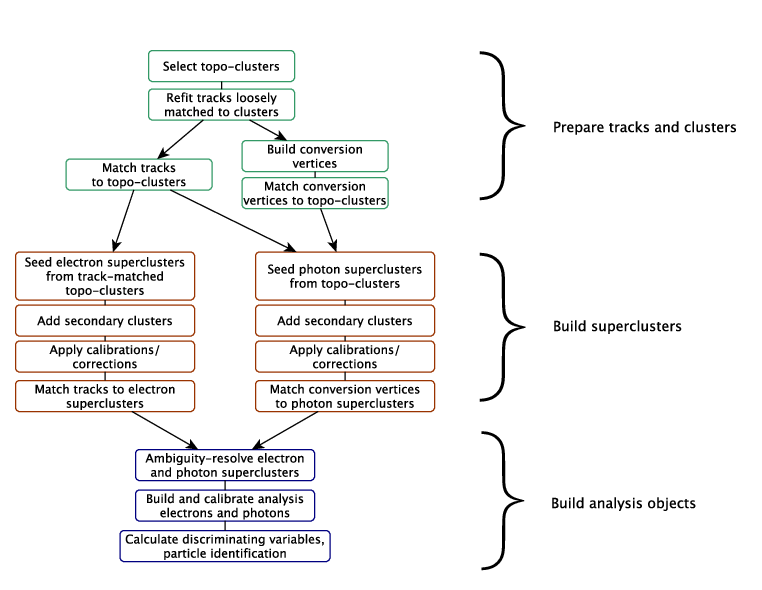
\includegraphics[width=.65\textwidth,keepaspectratio=true]{chapters/chapter5_eventreconnstruction/images/egamma_flow_01.png}
		\caption{\label{fig:egamma-reco} Algorithm flow diagram for the electron and photon reconstruction \cite{electron-perf}.}
		\end{figure}

	\section{Jets}\label{sec:reco-jets}
		A jet is a reconstructed object of calorimeter energy\footnote{The jet objects in this dissertation use the particle flow algorithm that includes track objects in the full jet energy calculation.} that is meant to capture the energy and direction of a hadronic shower, typically initiated from hard scatter quarks, hadrons, or gluons. There are several algorithms available to perform a clustering of calorimeter topoclusters to form jets. This dissertation uses jets created from particle flow objects. The particle flow algorithm is described in detail in Ref. \cite{pflow}, a flow chart of the algorithm is shown in Figure \ref{fig:pflow-flowchart} and an idealized example of the particle flow algorithm performing the reconstruction of hadrons is shown in Figure \ref{fig:pflow-example}. 

		\begin{figure}[!ht]
		\centering
		
\includegraphics[width=\textwidth,keepaspectratio=true]{chapters/chapter5_eventreconnstruction/images/pflow_flow_chart.png}
		\caption{\label{fig:pflow-flowchart} A flow chart of how the particle flow algorithm proceeds, starting with track selection and continuing until the energy associated with the selected tracks has been removed from the calorimeter. At the end, charged particles, topoclusters which have not been modified by the algorithm, and remnants of topoclusters which have had part of their energy removed remain \cite{pflow}.}
		\end{figure}

		\begin{figure}[!ht]
		\centering
		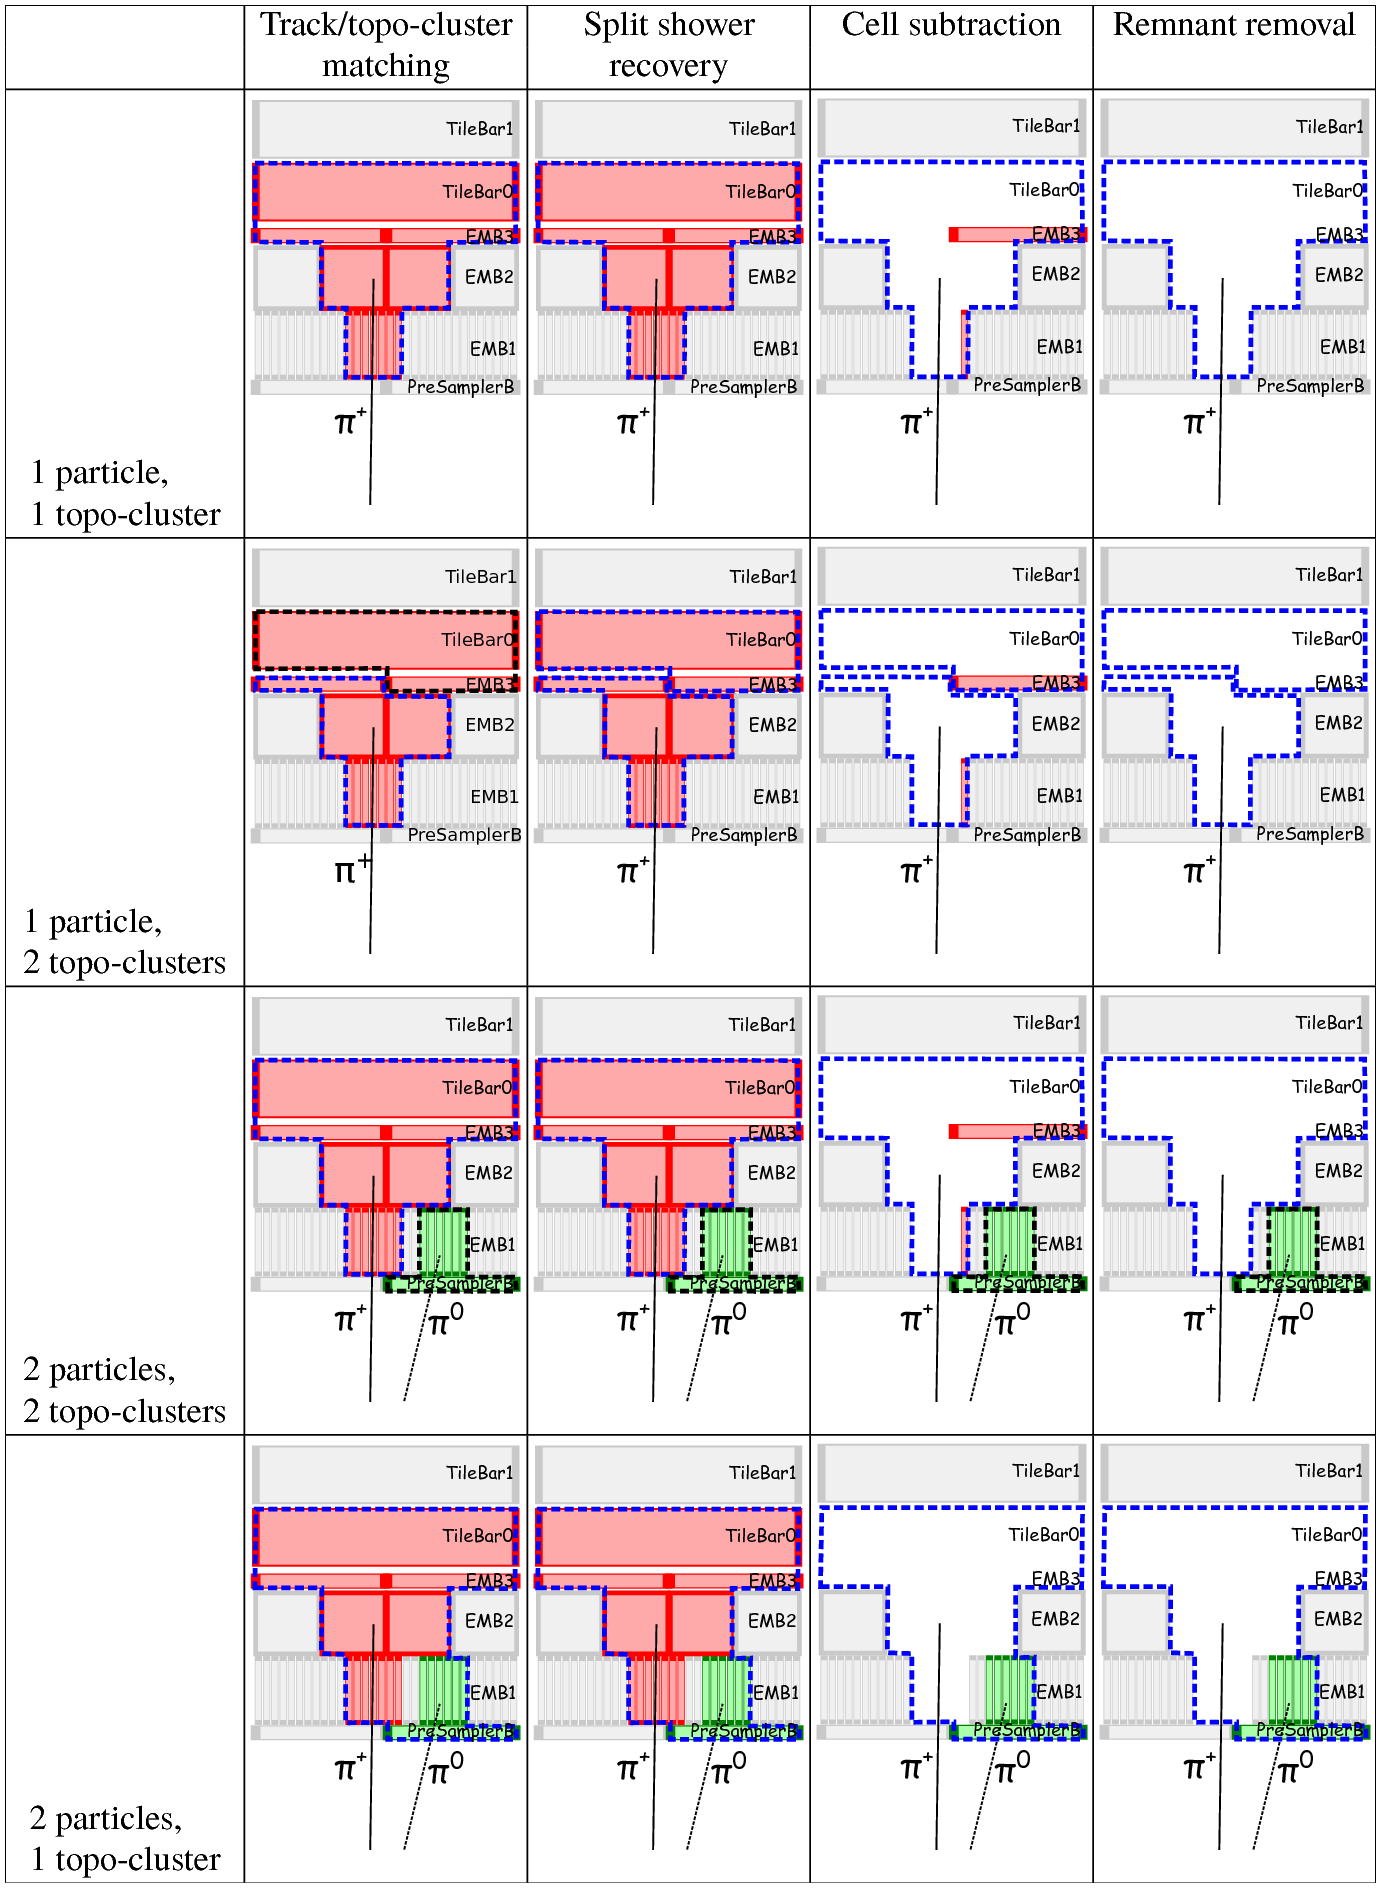
\includegraphics[width=.75\textwidth,keepaspectratio=true]{chapters/chapter5_eventreconnstruction/images/pflow_example.png}
		\caption{\label{fig:pflow-example} Idealized examples of how the algorithm is designed to deal with several different cases. The red cells are those which have energy from the $\pi^{+}$, the green have cells energy from the photons in the $\pi^{0}$  decay, the dotted lines represent the original topocluster boundaries with those outlined in blue having been matched by the algorithm to the $\pi^{+}$, while those in black are yet to be selected. The different layers in the EM calorimeter (Presampler, EMB1, EMB2, EMB3) are indicated. In this sketch only the first two layers of the Tile calorimeter are shown (TileBar0 and TileBar1) \cite{pflow}.}
		\end{figure}

		The particle flow algorithm starts by matching selected tracks to a single topocluster. The expected energy of the initial particle in the calorimeter is calculated from the track momentum and the topocluster position. The probability of the track-topocluster system being deposited in multiple topoclusters is then calculated. The algorithm then adds in more topoclusters to the output object based on this probability. The expected energy of the initial particle is subtracted from the energy of the matched topoclusters cell by cell. If the energy of the output object is consistent with a single particle signal, then the remaining topocluster remnants are removed. The outputs of the particle flow algorithm are then fed into the anti-$k_t$ algorithm \cite{anti-kt} with a radius value of $R=0.4$. 

		The anti-$k_t$ algorithm is a jet finding algorithm that is collinear and infrared safe, meaning the number of identified jets does not change due to splitting or merging of high transverse momentum particles, nor the presence of soft gluon emission between jets \cite{Cacciari_2008}. A jet is constructed in the anti-$k_t$ algorithm through an iterative process using a the distance parameter defined as 

		\begin{equation}\label{eqn:anti-kt-distance}
		d_{ij} = min(k_{t,i}^{-2} , k_{t,j}^{-2}) \frac{\Delta_{ij}^{2}}{R^2} 
		\end{equation}
		where $k_t$ is the transverse momentum, R is an input parameter defining the radius of the jet cone, and $\Delta_{ij}$ is the distance between objects $i$ and $j$ defined as
		\begin{equation}\label{eqn:anti-kt-delta}
		\Delta{ij} = (y_i - y_j)^2 + (\phi_i - \phi_j)^2
		\end{equation}
		The anti-kt algorithm first identifies the smallest $d_ij$ and clusters the particle flow objects if $d_{ij}>k_{t,i}^{-2}$. If $d_{ij}>k_{t,i}^{-2}$ then the particle flow object is discarded. This process continues iteratively until there are no more objects to consider. Objects with $\Delta>R$ are still considered, making the R input parameter an energy cut-off for clustering and not a direct radius value. Figure \ref{fig:anti-kt-comparison} shows the anti-$k_{t}$ algorithm's performance compared to other jet finding algorithms. The anti-$k_{t}$ algorithm results in a more conical shape than other jet finding algorithms; better encapsulating the shower profile of jets.

		\begin{figure}[!ht]
		\centering
		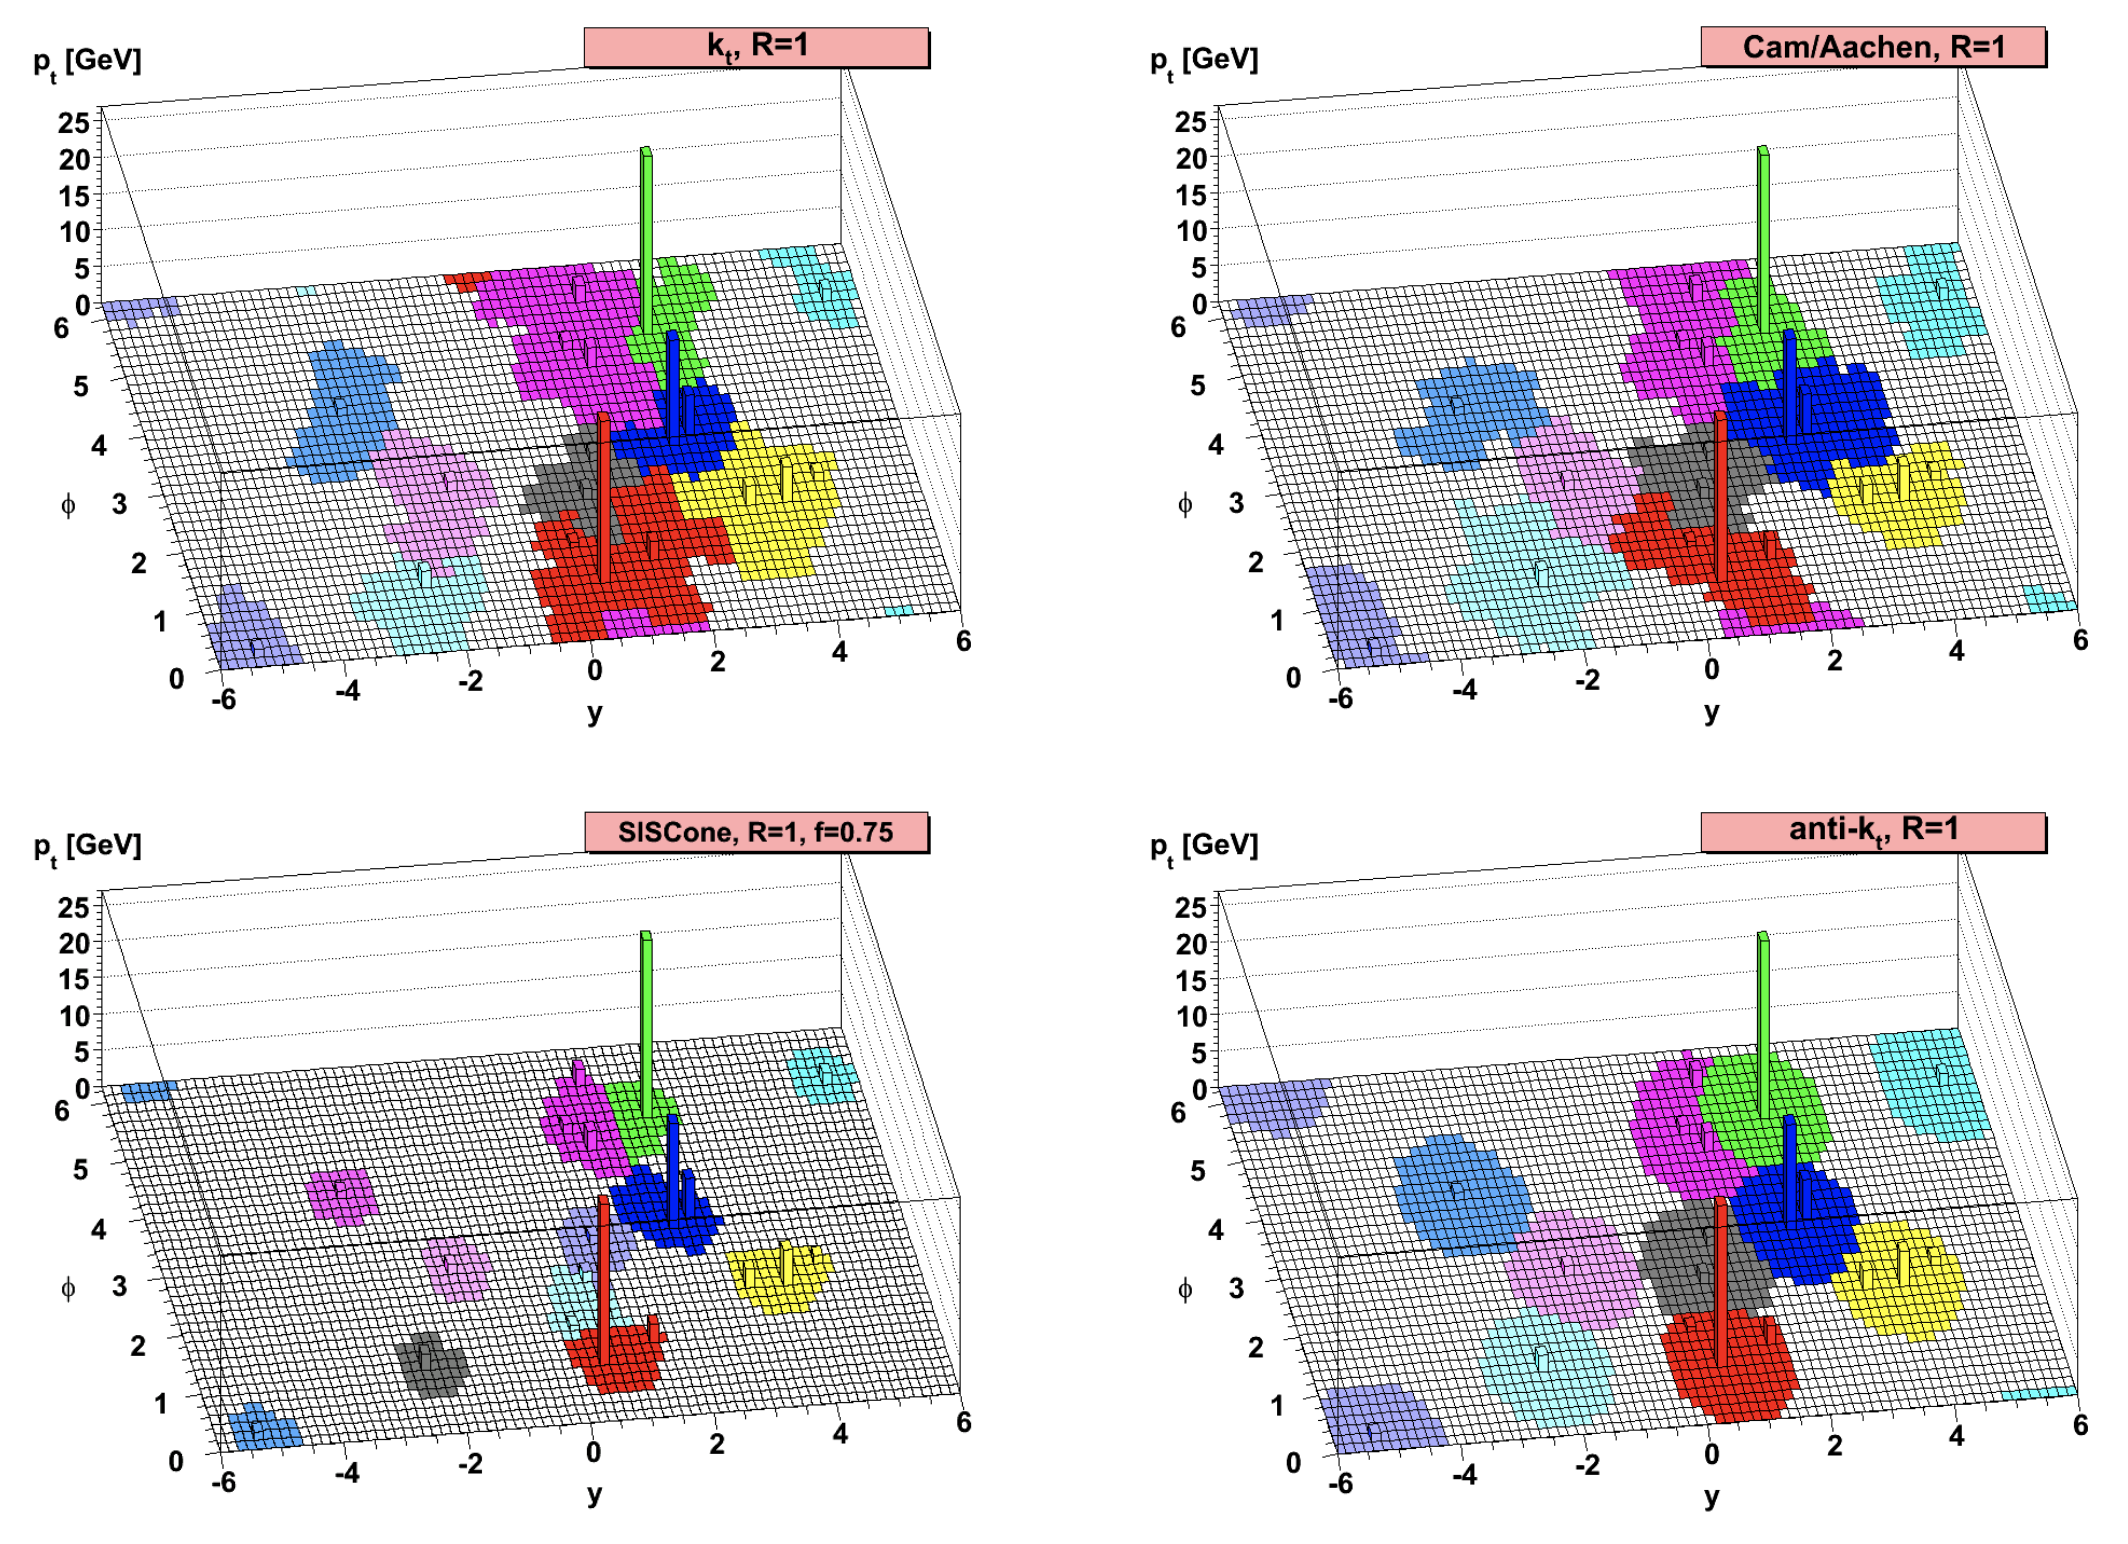
\includegraphics[width=.5\textwidth,keepaspectratio=true]{chapters/chapter5_eventreconnstruction/images/anti-kt-comparison.png}
		\caption{\label{fig:anti-kt-comparison} Comparison between several jet finding algorithms \cite{anti-kt}.}
		\end{figure}

		\textcolor{red}{Talk about jet calibration}

		\subsection{\bjet Tagging}\label{ssec:flavor-tagging}
			Jets originating from hard scatter b quarks are an important signature in high energy physics colliders, especially so in the analysis discussed in this dissertation. An initial state b quark hadronizes into B-hadrons which have a relatively long lifetime. Due to the relativistic speeds and long lifetime of the B-hadrons they travel a distance away from the \gls{IP} before decaying and creating a hadronic shower. This leads to a secondary vertex that can be measured. A pictorial representation is shown in Figure \ref{fig:bjet}. The impact parameter $d_0$ shown is the minimum distance between the tracks from the secondary vertex and \gls{IP}. 

			\begin{figure}[!ht]
			\centering
			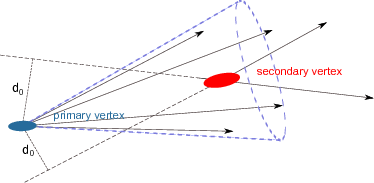
\includegraphics[width=.5\textwidth,keepaspectratio=true]{chapters/chapter5_eventreconnstruction/images/b-jet-schetch.png}
			\caption{\label{fig:bjet} Schematic view of the tracks in a \bjet \cite{bjet-trigger}.}
			\end{figure}

			There are several methods used to tag a jet as coming from a b quark; this analysis uses the DL1 high level tagger \cite{b-tagging} that is based on an artificial deep neural network. Neural networks are discussed in detail in Section \ref{sec:mva}. DL1 not only tags \bjets, but also outputs the probability for a jet to be initiated from a charm or light flavor quark. The DL1 tagger has over 20 input variables, including the $\pt$ and $\eta$ of jets \textcolor{red}{Find reference about DL1 inputs.} \cite{b-tagging-input-variables}. The analysis discussed in this dissertation uses a fixed cut working point that corresponds to an average efficiency of 70\% for \bjets in \ttbar events. \textcolor{red}{Quote light and c miss-tag rates.}


	\section{$\tau$ Identification}\label{ssec:reco-tau}
		One of the most important particles in the final state of the search discussed in this dissertation is the $\tau$ lepton. The decay channels of $\tau$ leptons make them difficult to reconstruct. A $\tau$ lepton can decay to hadrons, an electron, or a muon; in each decay mode, at least one neutrino is also present. The analysis discussed in this dissertation only considers $\tau$ leptons that have decayed hadronically. The hadronic decay mode consists of 1 or 3 charged hadrons ($\pi^{\pm}$), a neutrino, and possible neutral hadrons ($\pi^0$). A $\tau$ lepton decaying in this manner within the \gls{ATLAS} detector leaves 1 or 3 tracks in the \gls{ID} and collimated showers of energy in the calorimeters; the neutrino does not interact with the \gls{ATLAS} detector, therefore no direct signature is left behind. Reconstruction is done on the visible part of the hadronically decaying $\tau$ lepton, further referred to as \tauhad in the rest of this dissertation. 

		The \tauhad candidates start with an anti-$k_t$ jet seed with $E_T>10$ GeV in the calorimeter; tracks and topoclusters within $\Delta R = 0.2$ are added to the \tauhad candidate. The axis of the original jet seed is redefined in the direction of the \tauhad candidate and calibration is done at the \tauhad scale \cite{tau-id-calib}. An overlap removal is done to ensure the \tauhad candidate is isolated from electrons and muons. Tracks are required to have $E_{T}>30$ GeV, $|\eta|<2.3$ and strictly either 1 or 3 tracks. A \tauhad candidate is referred to as 1-prong or 3-prong based on the associated number of tracks. To discern \tauhad objects from quark-initiated and gluon-initiated jets a \gls{RNN} is used \cite{tau-id-rnn}. The search described in this analysis uses a medium \gls{WP} that corresponds to 75\% identification efficiency for 1-prong and 60\% for 3-prong in $\gamma \to \tau \tau$ collision events.

	\section{\Etm}\label{sec:reco-etmiss}
		The final \acrshort{SM} particle in the reconstruction scheme is the neutrino\footnote{The W, Z and gluon do not have long enough lifetimes to leave signatures within the \gls{ATLAS} detector volume. Instead, their presence is inferred through their decay products}. The presence of a neutrino, or another minimally interacting particle, can be inferred through the calculation of \Etm\footnote{The choice of \Etm to represent missing transverse momentum is a common nomenclature. Other choices include $\pt^{miss}$, MET, and et miss.}; which takes advantage of the initial collision having a small momentum in the transverse plane ($\pt \simeq 0$). The initial momentum in the z direction (along the beamline) cannot be known due to the composite nature of the colliding protons and the associated PDFs of their components.

		The calculation of \Etm in the \gls{ATLAS} detector is defined as
		\begin{equation}\label{eqn:etmiss}
		E_{T}^{miss} = - \sum E_{T} = \sum \pt^{\mu} + \sum \pt^{e} + \sum \pt^{\gamma} + \sum \pt^{\tau} + \sum \pt^{jets} + \sum \pt^{soft}
		\end{equation}
		where the $\pt^{soft}$ term comes from soft tracks that are not associated with any physics objects \cite{met-perf}. The analysis discussed in this dissertation uses \Etm triggers in one of the subchannels to select events and is described in Chapter \ref{chap:hpana}.